\section{Additional results}
\label{app:extra}
Table~\ref{tab:position} positions recent recovery work; Tables~\ref{tab:stress} and~\ref{tab:pop} give the stress and calibration-population results of RQ4 and RQ5;
Table~\ref{tab:seedvariance} reports variability across the \SimSeedCount{} fixed reporting seeds.
Table~\ref{tab:lag} prices the lag share; Table~\ref{tab:corr} gives the correlated-read experiment of RQ2; Table~\ref{tab:apps} lists testbed apps; Table~\ref{tab:realcone}
gives campaign~1 of the emulator measurements.
Figure~\ref{fig:sprt} and Table~\ref{tab:sprt} check Theorem~\ref{thm:main}(a,c) for an i.i.d.\ probe (all 24 cells; Monte Carlo means match the exact $\bar N$ to \SprtMCdev reads;
the strict thresholds over-deliver by up to \SprtSlackMax$\times$, median \SprtSlackMed$\times$); Table~\ref{tab:calib} shows calibration of one i.i.d.\ probe (Lemma~\ref{lem:calib}(i));
Figure~\ref{fig:floor} checks Theorem~\ref{thm:main}(d) (\ImpViol of 54 policy--prior cells below the floor beyond Monte Carlo error); Table~\ref{tab:nonce} validates Lemma~\ref{lem:nonce};
Table~\ref{tab:saga} details the saga allocation; Table~\ref{tab:sens} varies the simulator's free app parameters.

\begin{table}[t]
\centering
\caption{Misspecification and stress (model-based simulation, 12{,}000 paired workflows per row; the generative model departs from
the planner's assumptions as listed). $P_{\mathrm{v}}$: \% of committed effects retried by the planner (budget 1\%; CP 95\% upper bound in
parentheses); $L_{\mathrm{v}}$: \% of absent effects the planner declared done; ask: \% of workflows. Rules: the same-evidence rule baseline.}
\label{tab:stress}
\footnotesize
\setlength{\tabcolsep}{2pt}
\begin{tabular}{@{}l cc ccc@{}}
\toprule
 & Re-read & Rules & \multicolumn{3}{c}{\alg (product)} \\
\cmidrule(l){4-6}
Generative model & $P_{\mathrm{v}}$ & $P_{\mathrm{v}}$ & $P_{\mathrm{v}}$ (hi) & $L_{\mathrm{v}}$ & ask \\
\midrule
independent re-reads & 0.04 & 0.35 & 0.05 (0.12) & 0.00 & 21.5 \\
\quad + persistent nonce misses & 0.42 & 0.36 & 0.02 (0.09) & 0.02 & 21.9 \\
default world (Table~\ref{tab:planner}) & 3.69 & 0.52 & 0.05 (0.12) & 0.00 & 24.9 \\
cross-view VLM correlation 0.3 & 4.15 & 0.67 & 0.01 (0.07) & 0.00 & 26.7 \\
heavy lag tail, \emph{not} in calibration & 4.55 & 0.95 & 0.98 (1.22) & 0.00 & 25.6 \\
heavy lag tail, in calibration & 4.55 & 0.95 & 0.05 (0.12) & 0.00 & 48.7 \\
G2 broken (retry cap / force-stop) & 3.84 & 0.53 & 0.02 (0.09) & 0.00 & 26.2 \\
classified G2, server without dedup & 3.69 & 0.52 & 0.05 (0.12) & 0.00 & 24.9 \\
delayed recovery in Doze, not detected & 11.20 & 8.03 & 5.83 (6.36) & 0.00 & 25.2 \\
delayed recovery in Doze, detected & 11.20 & 8.03 & 0.00 (0.05) & 0.02 & 46.1 \\
stale history, 0.5\% common mode & 3.96 & 0.73 & 0.19 (0.31) & 0.02 & 25.2 \\
Monitor misreads 5\% of terminal states & 3.69 & 0.37 & 0.05 (0.12) & 0.00 & 25.6 \\
user wrong on 20\% of asks & 3.69 & 0.52 & 0.05 (0.12) & 0.00 & 24.9 \\
combined & 11.45 & 8.78 & 0.42 (0.58) & 0.00 & 47.9 \\
\bottomrule
\end{tabular}
\end{table}

\begin{table}[t]
\centering
\caption{Calibration population, common mode and calibration size (model-based simulation, 12{,}000 paired workflows per row). Cells: $P_{\mathrm{v}}$ (\%, budget 1\%) /
escalations (\%). Interrupted world: 2\% stale history after a restart, 3\% optimistic ``sending'' entries for tapped-but-uncommitted effects, 20\% heavy-tailed lags.
Passive labels come from uninterrupted effects; fault-injected labels from the interrupted population. Rules: $P_{\mathrm{v}}$ of the same-evidence rule baseline.}
\label{tab:pop}
\footnotesize
\setlength{\tabcolsep}{2pt}
\begin{tabular}{@{}l ccc c@{}}
\toprule
 & product & source & joint & rules \\
\midrule
default world, passive labels & 0.05 / 25 & 0.00 / 47 & 0.05 / 67 & 0.52 \\
interrupted world, passive labels & 0.87 / 26 & 0.13 / 48 & 0.34 / 67 & 1.34 \\
interrupted world, fault-injected labels & 0.11 / 46 & 0.00 / 56 & 0.00 / 80 & 1.34 \\
stale history 0.5\%, fault-injected & 0.16 / 26 & 0.01 / 49 & 0.00 / 74 & 0.73 \\
stale history 2\%, fault-injected & 0.31 / 29 & 0.01 / 50 & 0.01 / 74 & 1.10 \\
stale history 5\%, fault-injected & 0.33 / 33 & 0.01 / 50 & 0.00 / 75 & 2.16 \\
\midrule
$n_{\mathrm{cal}}{=}100$ (default world) & 0.00 / 52 & 0.00 / 100 & 0.00 / 100 & -- \\
$n_{\mathrm{cal}}{=}200$ (default world) & 0.00 / 40 & 0.00 / 73 & 0.00 / 100 & -- \\
$n_{\mathrm{cal}}{=}500$ (default world) & 0.04 / 31 & 0.00 / 62 & 0.00 / 100 & -- \\
$n_{\mathrm{cal}}{=}1{,}000$ (default world) & 0.05 / 27 & 0.00 / 60 & 0.00 / 100 & -- \\
$n_{\mathrm{cal}}{=}2{,}000$ (default world) & 0.05 / 25 & 0.00 / 47 & 0.05 / 67 & -- \\
$n_{\mathrm{cal}}{=}5{,}000$ (default world) & 0.02 / 23 & 0.04 / 27 & 0.04 / 34 & -- \\
$n_{\mathrm{cal}}{=}10{,}000$ (default world) & 0.04 / 23 & 0.05 / 24 & 0.07 / 26 & -- \\
\bottomrule
\end{tabular}
\end{table}

\begin{table*}[t]
\centering
\caption{Across-seed variability of asking rates for Table~\ref{tab:planner} (model-based) and Table~\ref{tab:realsim} (measured-parameter) over \SimSeedCount{} seeds: mean $\pm$ sample standard deviation and range, in \%. Element rows use 2{,}000 labels per class and outcome and 20{,}000 lag entries, so the vetted-rule row is not the matched case of Table~\ref{tab:matched}.}
\label{tab:seedvariance}
\small
\begin{tabular}{@{}llrr@{}}
\toprule
Profile & Policy & ask mean $\pm$ SD & ask range \\
\midrule
model & redo & 0.00 $\pm$ 0.00 & 0.00 to 0.00 \\
model & theorem-only & 72.98 $\pm$ 0.88 & 71.96 to 74.33 \\
model & always-ask & 100.00 $\pm$ 0.00 & 100.00 to 100.00 \\
model & rules & 23.90 $\pm$ 1.20 & 22.46 to 25.08 \\
model & product & 24.85 $\pm$ 1.29 & 23.21 to 26.58 \\
model & joint & 66.72 $\pm$ 0.94 & 65.38 to 67.67 \\
element & product & 3.01 $\pm$ 0.26 & 2.67 to 3.38 \\
element & joint & 72.86 $\pm$ 1.01 & 71.54 to 74.00 \\
element & vetted rules & 5.29 $\pm$ 6.80 & 2.17 to 17.46 \\
k9 & product & 100.00 $\pm$ 0.00 & 100.00 to 100.00 \\
k9 & joint & 100.00 $\pm$ 0.00 & 100.00 to 100.00 \\
k9sent & product & 100.00 $\pm$ 0.00 & 100.00 to 100.00 \\
k9sent & joint & 100.00 $\pm$ 0.00 & 100.00 to 100.00 \\
\bottomrule
\end{tabular}
\end{table*}

The relatively large Element vetted-rule standard deviation is driven by one reporting seed; the others cluster near the same low asking rate. This is seed variability in the fixed reporting runs, not a change to the pooled result.
\begin{table}[!htbp]
\centering
\caption{Wait for the lag tail to use at most $\alpha_{\mathrm{lag}}$ (Theorem~\ref{thm:main}(a,b)): exact quantile $G^{-1}(\alpha_{\mathrm{lag}})$ and the wait certified from 20{,}000 logged lags (one-sided CP, $\delta{=}10^{-4}$), with the median and shape of $T$ per row. A dash: not certifiable with 20{,}000 samples.}
\label{tab:lag}
\footnotesize
\setlength{\tabcolsep}{3pt}
\begin{tabular}{@{}l cc cc@{}}
\toprule
 & \multicolumn{2}{c}{$\alpha_{\mathrm{lag}}{=}10^{-2}$} & \multicolumn{2}{c}{$\alpha_{\mathrm{lag}}{=}10^{-3}$} \\
\cmidrule(lr){2-3}\cmidrule(l){4-5}
Lag $T$ & exact & certified & exact & certified \\
\midrule
lognormal, 1.5\,s, $\sigma{=}0.6$ & 6\,s & 7\,s & 10\,s & 12\,s \\
lognormal, 3\,s, $\sigma{=}1.2$ & 49\,s & 57\,s & 2\,min & 3\,min \\
Pareto, 1\,s, $\kappa{=}3$ & 5\,s & 5\,s & 10\,s & 16\,s \\
Pareto, 2\,s, $\kappa{=}1.1$ & 2\,min & 3\,min & 18\,min & 98\,min \\
\bottomrule
\end{tabular}
\end{table}

\begin{table}[!htbp]
\centering
\caption{Correlated reads (model-based simulation; VLM family of 3 views, $\epsilon{=}0.10$, $\alpha{=}1\%$, 30{,}000 committed effects per cell): $P(\mathrm{dup}\mid X{=}1)$ in \%. Within-view: re-reads share one error with probability $\rho$. Cross-view: views share a latent rate with correlation $\rho$. naive: SPRT on one view; re-read: SPRT over rotated re-reads; view: one read per view; certified: family bound (Prop.~\ref{prop:family}), asks in parentheses; bound: Lemma~\ref{lem:floor}.}
\label{tab:corr}
\footnotesize
\setlength{\tabcolsep}{2pt}
\begin{tabular}{@{}c ccc cccc@{}}
\toprule
 & \multicolumn{3}{c}{Within-view $\rho$} & \multicolumn{4}{c}{Cross-view $\rho$} \\
\cmidrule(lr){2-4}\cmidrule(l){5-8}
$\rho$ & naive & re-read & view & re-read & view & certified & bound \\
\midrule
0.0 & 0.12 & 0.16 & 0.11 & 0.13 & 0.11 & 0.06 (27) & 0.1 \\
0.2 & 2.13 & 0.36 & 0.09 & 3.19 & 1.13 & 0.00 (100) & 2.2 \\
0.6 & 5.95 & 0.99 & 0.09 & 8.42 & 5.03 & 0.00 (100) & 6.3 \\
1.0 & 9.63 & 1.89 & 0.11 & 10.21 & 10.39 & 0.00 (100) & 10.0 \\
\bottomrule
\end{tabular}
\end{table}

\begin{table}[!htbp]
\centering
\caption{Testbed apps. Dedup basis from protocol specifications~\cite{matrix_spec,rfc4791,rfc9110,rfc5321}, nonce field from the app's UI. \emph{Measured}: on our emulator testbed (Table~\ref{tab:real}); \emph{planned}: not yet measured. K-9's nonce is the visible subject, used only on opted-in test accounts.}
\label{tab:apps}
\footnotesize
\setlength{\tabcolsep}{2pt}
\resizebox{\columnwidth}{!}{%
\begin{tabular}{@{}lll l l@{}}
\toprule
App & Backend & Hop-2 dedup basis & Nonce field & Status \\
\midrule
Element & Synapse & Matrix txnId & body (visible) & measured \\
Etar + DAVx5 & Radicale & URL + If-None-Match & event description & measured \\
Tasks.org + DAVx5 & Radicale & URL + If-None-Match & task note & planned \\
Joplin & WebDAV & \texttt{PUT} by note id & note body & planned \\
K-9 Mail 24.0 & GreenMail & none (SMTP) & subject (visible) & measured \\
Simple SMS & SMS & none & body (visible) & planned \\
MockBank-A / B & ours & request id / none & private note & planned \\
Pro Expense & local & n/a & note & planned \\
Markor & local & n/a & file & planned \\
\bottomrule
\end{tabular}}
\end{table}

\begin{table}[!htbp]
\centering
\caption{Campaign 1 (superseded by Table~\ref{tab:real} for lags and family errors): hop-2 behaviour of Element~1.6.62 and K-9~Mail~24.0 over no kill, background + kill and force-stop, 45\,s window. Re-sent: request sent again (Element: same txnId); Once: one server copy; Later: after the run; Unsent: shown as unsent. No duplicate. Its reader had no screen check (\S\ref{sec:eval-real}).}
\label{tab:realcone}
\footnotesize
\setlength{\tabcolsep}{2.4pt}
\begin{tabular}{@{}l ccccc@{}}
\toprule
App, condition & $n$ & Re-sent & Once & Later & Unsent \\
\midrule
Element, response lost after commit & 14 & 14 & 14 & 14 & 0 \\
\quad offline before send & 14 & 0 & 13 & 14 & 0 \\
\quad SIGKILL 300\,ms after \emph{Send} & 5 & 0 & 5 & 5 & 0 \\
\quad acknowledged, then kill & 4 & 0 & 4 & 4 & 0 \\
K-9, response lost after commit & 15 & 0 & 15 & 15 & 15 \\
\quad offline before send & 15 & 0 & 2 & 15 & 13 \\
\quad acknowledged, then kill & 5 & 0 & 5 & 5 & 0 \\
\bottomrule
\end{tabular}
\end{table}

\begin{table}[t]
\caption{LLM-agent arms on the K-9 trap (LLM-agent experiment): valid over scheduled episodes, episodes in which K-9 sent mail
again after the restart (Resent), episodes with two tagged copies at the backend (Dup), Wilson 95\% interval for
the duplicate rate (\%), and asks. Each arm has its own freeze; arms ran one after the other.}
\label{tab:agent-arms}
\centering
\footnotesize
\setlength{\tabcolsep}{3pt}
\begin{tabular}{@{}llllccccc@{}}
\toprule
Agent & Fault & Sent folder & Recovery & Valid & Resent & Dup & 95\% CI & Asks \\
\midrule
M3A & force-stop & both & none (native) & 18/20 & 17 & 17 & [74.2, 99.0] & 0 \\
T3A & force-stop & both & none (native) & 10/23 & 9 & 3 & [10.8, 60.3] & 0 \\
M3A & agent kill only & both & none (native) & 19/20 & 19 & 19 & [83.2, 100.0] & 0 \\
M3A & force-stop & Sent & same-evidence rules & 15/20 & 14 & 14 & [70.2, 98.8] & 0 \\
M3A & force-stop & both & \sys & 19/20 & 1 & 1 & [0.9, 24.6] & 19 \\
\bottomrule
\end{tabular}
\end{table}

\begin{figure}[!htbp]
\centering
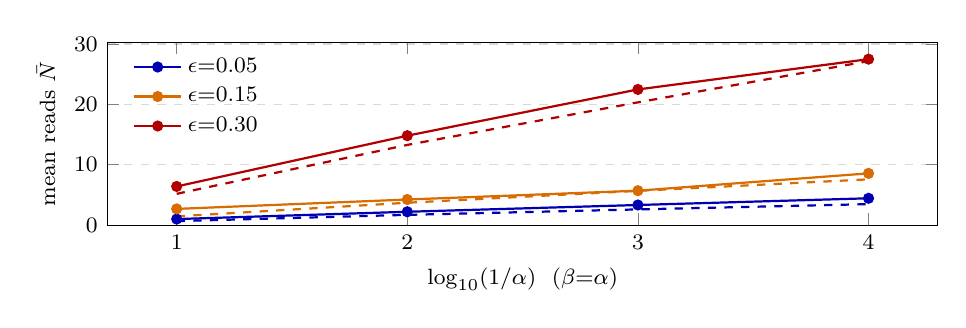
\begin{tikzpicture}
\begin{axis}[width=\linewidth,height=3.9cm,xlabel={$\log_{10}(1/\alpha)$ \ ($\beta{=}\alpha$)},
  ylabel={mean reads $\bar N$},xtick={1,2,3,4},ymin=0,
  legend style={at={(0.02,0.98)},anchor=north west,font=\footnotesize,draw=none,fill=none},
  ymajorgrids,grid style={dashed,gray!30},tick label style={font=\footnotesize},label style={font=\footnotesize}]
\addplot[color=blue!70!black,mark=*,mark size=1.6pt,thick] coordinates {(1,1.000) (2,2.210) (3,3.332) (4,4.444)};
\addlegendentry{$\epsilon{=}0.05$}
\addplot[color=blue!70!black,dashed,thick,forget plot] coordinates {(1,0.663) (2,1.699) (3,2.601) (4,3.475)};
\addplot[color=orange!85!black,mark=*,mark size=1.6pt,thick] coordinates {(1,2.685) (2,4.239) (3,5.703) (4,8.571)};
\addlegendentry{$\epsilon{=}0.15$}
\addplot[color=orange!85!black,dashed,thick,forget plot] coordinates {(1,1.448) (2,3.709) (3,5.677) (4,7.584)};
\addplot[color=red!70!black,mark=*,mark size=1.6pt,thick] coordinates {(1,6.405) (2,14.815) (3,22.478) (4,27.495)};
\addlegendentry{$\epsilon{=}0.30$}
\addplot[color=red!70!black,dashed,thick,forget plot] coordinates {(1,5.186) (2,13.287) (3,20.338) (4,27.170)};
\end{axis}
\end{tikzpicture}
\caption{The price of a duplicate budget for an i.i.d.\ probe (exact). Solid: SPRT; dashed: lower bound~\eqref{eq:lb}.
Cost grows as $\log(1/\alpha)/\mathrm{KL}$; the gap is at most 2.4 reads over all 24 cells (Table~\ref{tab:sprt}).}
\label{fig:sprt}
\end{figure}

\begin{table}[!htbp]
\centering
\caption{Implementation sanity check of Theorem~\ref{thm:main}(a,c) for an i.i.d.\ binary probe ($\epsilon_0{=}\epsilon_1{=}\epsilon$, $\beta{=}\alpha$), all 24 cells.
Exact DTMC values; ``MC hi'': one-sided 95\% Clopper--Pearson upper bound on $P(\mathrm{dup}\mid X{=}1)$ from 40{,}000 committed-world episodes;
$\bar N$: mean reads at $\pi{=}\tfrac12$, exact and MC; LB/UB: bounds~\eqref{eq:lb}/\eqref{eq:ub} averaged over the two outcomes.
At $\alpha{=}10^{-4}$, 40{,}000 episodes cannot confirm the budget by MC (zero events give an upper bound of $9.2{\times}10^{-5}$); the exact column does.}
\label{tab:sprt}
\footnotesize
\setlength{\tabcolsep}{3pt}
\begin{tabular}{@{}cc cc cccc@{}}
\toprule
$\epsilon$ & $\alpha$ & $P(\mathrm{dup})$ & MC hi & $\bar N$ & $\bar N_{\mathrm{MC}}$ & LB & UB \\
\midrule
0.05 & $10^{-1}$ & \ensuremath{0.05} & \ensuremath{0.05} & 1.00 & 1.00 & 0.66 & 1.98 \\
0.05 & $10^{-2}$ & \ensuremath{2.8{\times}10^{-3}} & \ensuremath{3.5{\times}10^{-3}} & 2.21 & 2.21 & 1.70 & 2.85 \\
0.05 & $10^{-3}$ & \ensuremath{1.5{\times}10^{-4}} & \ensuremath{2.2{\times}10^{-4}} & 3.33 & 3.33 & 2.60 & 3.72 \\
0.05 & $10^{-4}$ & \ensuremath{7.7{\times}10^{-6}} & \ensuremath{9.2{\times}10^{-5}} & 4.44 & 4.44 & 3.47 & 4.59 \\
0.10 & $10^{-1}$ & \ensuremath{0.01} & \ensuremath{0.01} & 2.44 & 2.44 & 1.00 & 2.56 \\
0.10 & $10^{-2}$ & \ensuremath{1.4{\times}10^{-3}} & \ensuremath{1.5{\times}10^{-3}} & 3.74 & 3.74 & 2.56 & 3.87 \\
0.10 & $10^{-3}$ & \ensuremath{1.5{\times}10^{-4}} & \ensuremath{2.2{\times}10^{-4}} & 5.00 & 4.99 & 3.92 & 5.18 \\
0.10 & $10^{-4}$ & \ensuremath{1.7{\times}10^{-5}} & \ensuremath{9.2{\times}10^{-5}} & 6.25 & 6.25 & 5.24 & 6.49 \\
0.15 & $10^{-1}$ & \ensuremath{0.03} & \ensuremath{0.03} & 2.68 & 2.69 & 1.45 & 3.32 \\
0.15 & $10^{-2}$ & \ensuremath{5.5{\times}10^{-3}} & \ensuremath{6.0{\times}10^{-3}} & 4.24 & 4.24 & 3.71 & 5.22 \\
0.15 & $10^{-3}$ & \ensuremath{9.7{\times}10^{-4}} & \ensuremath{1.2{\times}10^{-3}} & 5.70 & 5.70 & 5.68 & 7.12 \\
0.15 & $10^{-4}$ & \ensuremath{3.0{\times}10^{-5}} & \ensuremath{1.8{\times}10^{-4}} & 8.57 & 8.56 & 7.58 & 9.01 \\
0.20 & $10^{-1}$ & \ensuremath{0.06} & \ensuremath{0.06} & 2.94 & 2.94 & 2.11 & 4.43 \\
0.20 & $10^{-2}$ & \ensuremath{3.9{\times}10^{-3}} & \ensuremath{4.4{\times}10^{-3}} & 6.61 & 6.59 & 5.41 & 7.20 \\
0.20 & $10^{-3}$ & \ensuremath{9.8{\times}10^{-4}} & \ensuremath{1.3{\times}10^{-3}} & 8.32 & 8.32 & 8.29 & 9.97 \\
0.20 & $10^{-4}$ & \ensuremath{6.1{\times}10^{-5}} & \ensuremath{1.8{\times}10^{-4}} & 11.67 & 11.66 & 11.07 & 12.74 \\
0.25 & $10^{-1}$ & \ensuremath{0.04} & \ensuremath{0.04} & 5.57 & 5.56 & 3.20 & 6.19 \\
0.25 & $10^{-2}$ & \ensuremath{4.1{\times}10^{-3}} & \ensuremath{4.9{\times}10^{-3}} & 9.92 & 9.93 & 8.20 & 10.38 \\
0.25 & $10^{-3}$ & \ensuremath{4.6{\times}10^{-4}} & \ensuremath{1.0{\times}10^{-3}} & 13.99 & 13.99 & 12.55 & 14.58 \\
0.25 & $10^{-4}$ & \ensuremath{5.1{\times}10^{-5}} & \ensuremath{9.2{\times}10^{-5}} & 18.00 & 17.98 & 16.76 & 18.77 \\
0.30 & $10^{-1}$ & \ensuremath{0.07} & \ensuremath{0.08} & 6.41 & 6.38 & 5.19 & 9.29 \\
0.30 & $10^{-2}$ & \ensuremath{6.2{\times}10^{-3}} & \ensuremath{6.8{\times}10^{-3}} & 14.82 & 14.79 & 13.29 & 16.09 \\
0.30 & $10^{-3}$ & \ensuremath{4.9{\times}10^{-4}} & \ensuremath{8.0{\times}10^{-4}} & 22.48 & 22.47 & 20.34 & 22.88 \\
0.30 & $10^{-4}$ & \ensuremath{9.0{\times}10^{-5}} & \ensuremath{1.8{\times}10^{-4}} & 27.50 & 27.53 & 27.17 & 29.68 \\
\bottomrule
\end{tabular}
\end{table}

\begin{table}[!htbp]
\centering
\caption{Calibration of an i.i.d.\ binary probe (Lemma~\ref{lem:calib}(i)): share of probe types (\%) whose exact $P(\mathrm{dup}\mid X{=}1)$ or $P(\mathrm{loss}\mid X{=}0)$ exceeds 0.01, and mean reads, over 200 probe types $\times$ 5 seeds. CP: one-sided upper bounds at $1{-}\delta$.}
\label{tab:calib}
\footnotesize
\setlength{\tabcolsep}{3.5pt}
\begin{tabular}{@{}r cc cc cc@{}}
\toprule
 & \multicolumn{2}{c}{Plug-in} & \multicolumn{2}{c}{CP, $\delta{=}0.05$} & \multicolumn{2}{c}{CP, $\delta{=}\alpha/20$} \\
\cmidrule(lr){2-3}\cmidrule(lr){4-5}\cmidrule(l){6-7}
$n_{\mathrm{cal}}$ & viol. & $\bar N$ & viol. & $\bar N$ & viol. & $\bar N$ \\
\midrule
25 & 56.3 & 4.2 & 1.5 & 9.2 & 0.0 & 22.9 \\
50 & 44.1 & 4.3 & 1.6 & 7.0 & 0.0 & 13.3 \\
100 & 33.7 & 4.3 & 1.0 & 5.7 & 0.0 & 8.2 \\
200 & 19.2 & 4.3 & 0.7 & 5.2 & 0.0 & 6.5 \\
400 & 12.2 & 4.2 & 0.6 & 4.8 & 0.0 & 5.6 \\
\bottomrule
\end{tabular}
\end{table}

\begin{table}[!htbp]
\centering
\caption{Content-carried nonce (Lemma~\ref{lem:nonce}; simulated OCR with substitutions, insertions and deletions; edit-distance matching).
OCR symbol error $e_c$; false-match bound $\epsilon_0$; miss rate $\epsilon_1$ analytic bound (MC, 40{,}000 screens), of which $\eta{=}1\%$
is a \emph{persistent} hidden field; $\mathrm{KL}(p_0\|p_1)$; mean reads at $\alpha{=}\beta{=}10^{-3}$ \emph{if} re-reads were independent.
With persistent misses no number of nonce reads certifies ``absent'' below $\eta$ (Lemma~\ref{lem:floor}).}
\label{tab:nonce}
\footnotesize
\setlength{\tabcolsep}{2.4pt}
\begin{tabular}{@{}l c c c c c@{}}
\toprule
Probe & $e_c$ & $\epsilon_0$ & $\epsilon_1$ & KL$_0$ & $\bar N$ \\
\midrule
VLM, no look-alike & -- & 0.12 & 0.08 & 1.87 & 4.4 \\
VLM, look-alike & -- & \multicolumn{2}{c}{uninformative} & 0 & $\infty$ \\
\midrule
nonce $k{=}4$, $t{=}0$ & 2\% & \ensuremath{3.8{\times}10^{-5}} & 0.087 (0.088) & 2.44 & 2.1 \\
nonce $k{=}4$, $t{=}0$ & 5\% & \ensuremath{3.8{\times}10^{-5}} & 0.194 (0.187) & 1.64 & 3.1 \\
nonce $k{=}6$, $t{=}1$ & 2\% & \ensuremath{7.2{\times}10^{-6}} & 0.016 (0.015) & 4.16 & 1.5 \\
nonce $k{=}6$, $t{=}1$ & 5\% & \ensuremath{7.2{\times}10^{-6}} & 0.042 (0.040) & 3.16 & 2.0 \\
nonce $k{=}8$, $t{=}1$ & 2\% & \ensuremath{9.3{\times}10^{-9}} & 0.020 (0.020) & 3.90 & 1.5 \\
nonce $k{=}8$, $t{=}1$ & 5\% & \ensuremath{9.3{\times}10^{-9}} & 0.067 (0.066) & 2.71 & 2.0 \\
\bottomrule
\end{tabular}
\end{table}

\begin{figure}[!htbp]
\centering
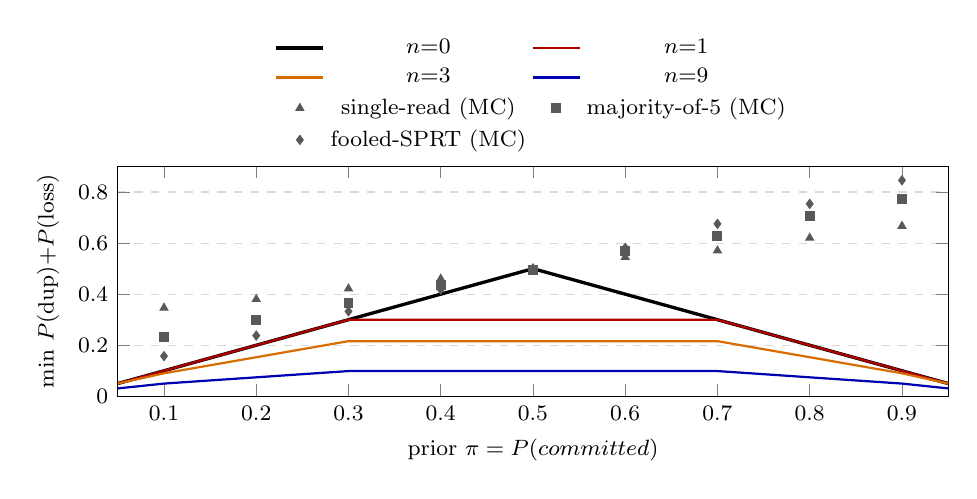
\begin{tikzpicture}
\begin{axis}[width=\linewidth,height=4.5cm,xlabel={prior $\pi=P(\text{committed})$},ylabel={min $P(\mathrm{dup}){+}P(\mathrm{loss})$},
  ymin=0,ymax=0.9,xmin=0.05,xmax=0.95,legend columns=2,
  legend style={at={(0.5,1.02)},anchor=south,font=\footnotesize,draw=none,fill=none},
  ymajorgrids,grid style={dashed,gray!30},tick label style={font=\footnotesize},label style={font=\footnotesize}]
\addplot[color=black,very thick] coordinates {(0.05,0.0500) (0.10,0.1000) (0.15,0.1500) (0.20,0.2000) (0.25,0.2500) (0.30,0.3000) (0.35,0.3500) (0.40,0.4000) (0.45,0.4500) (0.50,0.5000) (0.55,0.4500) (0.60,0.4000) (0.65,0.3500) (0.70,0.3000) (0.75,0.2500) (0.80,0.2000) (0.85,0.1500) (0.90,0.1000) (0.95,0.0500)};
\addlegendentry{$n{=}0$}
\addplot[color=red!70!black,thick] coordinates {(0.05,0.0500) (0.10,0.1000) (0.15,0.1500) (0.20,0.2000) (0.25,0.2500) (0.30,0.3000) (0.35,0.3000) (0.40,0.3000) (0.45,0.3000) (0.50,0.3000) (0.55,0.3000) (0.60,0.3000) (0.65,0.3000) (0.70,0.3000) (0.75,0.2500) (0.80,0.2000) (0.85,0.1500) (0.90,0.1000) (0.95,0.0500)};
\addlegendentry{$n{=}1$}
\addplot[color=orange!85!black,thick] coordinates {(0.05,0.0500) (0.10,0.0900) (0.15,0.1215) (0.20,0.1530) (0.25,0.1845) (0.30,0.2160) (0.35,0.2160) (0.40,0.2160) (0.45,0.2160) (0.50,0.2160) (0.55,0.2160) (0.60,0.2160) (0.65,0.2160) (0.70,0.2160) (0.75,0.1845) (0.80,0.1530) (0.85,0.1215) (0.90,0.0900) (0.95,0.0500)};
\addlegendentry{$n{=}3$}
\addplot[color=blue!70!black,thick] coordinates {(0.05,0.0309) (0.10,0.0498) (0.15,0.0621) (0.20,0.0743) (0.25,0.0866) (0.30,0.0988) (0.35,0.0988) (0.40,0.0988) (0.45,0.0988) (0.50,0.0988) (0.55,0.0988) (0.60,0.0988) (0.65,0.0988) (0.70,0.0988) (0.75,0.0866) (0.80,0.0743) (0.85,0.0621) (0.90,0.0498) (0.95,0.0309)};
\addlegendentry{$n{=}9$}
\addplot[only marks,mark=triangle*,mark size=1.6pt,gray!70!black] coordinates {(0.10,0.3462) (0.20,0.3804) (0.30,0.4217) (0.40,0.4600) (0.50,0.4982) (0.60,0.5452) (0.70,0.5706) (0.80,0.6202) (0.90,0.6668)};
\addlegendentry{single-read (MC)}
\addplot[only marks,mark=square*,mark size=1.6pt,gray!70!black] coordinates {(0.10,0.2336) (0.20,0.2999) (0.30,0.3656) (0.40,0.4355) (0.50,0.4951) (0.60,0.5691) (0.70,0.6267) (0.80,0.7063) (0.90,0.7709)};
\addlegendentry{majority-of-5 (MC)}
\addplot[only marks,mark=diamond*,mark size=1.6pt,gray!70!black] coordinates {(0.10,0.1573) (0.20,0.2379) (0.30,0.3327) (0.40,0.4179) (0.50,0.5008) (0.60,0.5814) (0.70,0.6753) (0.80,0.7537) (0.90,0.8462)};
\addlegendentry{fooled-SPRT (MC)}
\end{axis}
\end{tikzpicture}
\caption{Sanity check of Theorem~\ref{thm:main}(d). Lines: exact Bayes floor $\mathbb{E}[\min(\pi_n,1{-}\pi_n)]$ after $n$ reads of an
informative probe ($\epsilon{=}0.3$). Markers: policies against an \emph{uninformative} probe (20{,}000 episodes each); none goes below $n{=}0$.}
\label{fig:floor}
\end{figure}

\begin{table}[!htbp]
\centering
\caption{Saga budget allocation (Proposition~\ref{prop:saga}), $\alpha{=}\beta{=}0.01$, 200 random i.i.d.-probe workflows per $k$ (exact DP).
Mean reads under uniform and KKT splits, mean saving (\%) measured and predicted, share of workflows (\%) where KKT is \emph{worse} than uniform in
exact cost, worst end-to-end $P(\mathrm{dup})$ (\%) with KKT, and with every step given the full $\alpha$.}
\label{tab:saga}
\footnotesize
\setlength{\tabcolsep}{2.6pt}
\begin{tabular}{@{}r cc cc c cc@{}}
\toprule
$k$ & uniform & KKT & saving & pred. & worse & e2e dup & full-$\alpha$ \\
\midrule
2 & 12.4 & 12.2 & 0.95 & 0.95 & 38 & 0.86 & 1.5 \\
4 & 26.0 & 25.6 & 1.40 & 1.38 & 26 & 0.73 & 2.8 \\
8 & 59.2 & 58.3 & 1.52 & 1.49 & 8 & 0.68 & 5.3 \\
16 & 126.6 & 124.7 & 1.51 & 1.48 & 4 & 0.62 & 9.6 \\
\bottomrule
\end{tabular}
\end{table}

\begin{table}[!htbp]
\centering
\caption{Sensitivity to the simulator's free app-profile parameters (4{,}800 paired workflows per row). Cells: dup+loss (\% of workflows) /
escalations (\%); last column: GhostEffect's $P_{\mathrm{v}}$ (\%, budget 1\%) with its 95\% CP upper bound.}
\label{tab:sens}
\footnotesize
\setlength{\tabcolsep}{2.2pt}
\begin{tabular}{@{}l cccc c@{}}
\toprule
Variant & key & nonce+ask & always ask & GhostEffect & $P_{\mathrm{v}}$ (hi) \\
\midrule
default & 9.1 / 0 & 6.2 / 14 & 6.7 / 100 & 1.7 / 24 & 0.09 (0.26) \\
look-alikes x0.5 & 8.8 / 0 & 6.1 / 14 & 6.2 / 100 & 1.3 / 23 & 0.09 (0.26) \\
look-alikes x2 & 10.8 / 0 & 6.1 / 14 & 7.8 / 100 & 2.1 / 26 & 0.06 (0.22) \\
no nonce fields & 27.0 / 0 & 7.1 / 100 & 6.9 / 100 & 2.4 / 34 & 0.00 (0.11) \\
visible nonce opt-in & 9.1 / 0 & 6.2 / 14 & 7.0 / 100 & 1.5 / 18 & 0.06 (0.22) \\
no G2 apps & 4.8 / 0 & 1.6 / 15 & 7.6 / 100 & 2.0 / 27 & 0.03 (0.18) \\
G2 wherever hop-1 & 14.2 / 0 & 12.1 / 13 & 7.2 / 100 & 1.4 / 21 & 0.00 (0.11) \\
\bottomrule
\end{tabular}
\end{table}


\clearpage
